\chapter{Testing}
\begin{table}[h]
\begin{tabular}{|c|p{5cm}|p{5cm}|p{3cm}|}
  \hline
  Sr. No. & Scenario & Expected Result & Obtained Expected Results (True/False)\\
  \hline
  1 & Successfully load the shape file. & The JMapFrame is rendering the Map Properly. & True\\
  \hline
  2 & Successfully render Geo-referenced Raster data. & The JMapFrame is rendering the Image Properly. & True\\
  \hline
  3 & Load non-georeferenced Data. & Nothing is displayed in MapFrame. & True\\
  \hline
  4	& Selecting the feature. & The feature is colored in Map with different color and highlighted. & True\\
  \hline
  5 & Calculate the distance. & The output in kilometers is prompted in screen. & True\\
  \hline
  6 & Fetch the Attribute Table. & The attribute table is displayed on screen. & True\\
  \hline
  7 & Query perform on Attribute. & The desired output according to query is displayed. & True\\
  \hline
  \end{tabular}
  \end{table}
  \newpage
  \begin{table}[h]
  \begin{tabular}{|c|p{5cm}|p{5cm}|p{3cm}|}
  \hline
  Sr. No. & Scenario & Expected Result & Obtained Expected Results (True/False)\\
  \hline
  8 & Save the mapframe content as Image. & Prompt for option to save file in local directory and successfully save the file. & True\\
  \hline
  9 & Crop the geotiff image. & Ask for input of cropping parameter and perform according to that. & True\\
  \hline
  10 & Find the feature from Map. & Taking attribute name and its value and search it in table and highlight the area if desired result is got. & True\\
  \hline
  11 & Save as Shape file. & Ability to change CRS of Map and option to save the reprojected shape file. & True\\
  \hline
\end{tabular}
\caption[Test cases]{Test Cases}
\end{table}

\chapter{Future Enhancement}
 The application is Desktop GIS application, which user shape file or geo referenced jpg or tiff file. As enhancement geoserver can be included with this project. In computing, GeoServer - an open-source server written in Java - allows users to share and edit geospatial data. Designed for interpretability, it publishes data from any major spatial data source using open standards. GeoServer has evolved to become an easy method of connecting existing information to Virtual Globes such as Google Earth and NASA World Wind as well as to web-based maps such as OpenLayers, Google Maps and Bing Maps. GeoServer functions as the reference implementation of the Open Geospatial Consortium Wveb Feature Service standard, and also implements the Web Map Service and Web Coverage Service specifications.

GeoServer is the reference implementation of the Open Geospatial Consortium (OGC) Web Feature Service (WFS) and Web Coverage Service (WCS) standards, as well as a high performance certified compliant Web Map Service (WMS). GeoServer forms a core component of the Geospatial Web.

Something like Disaster management system using GIS can be made using this. To do this one need sensor which gives continuous information to us and when any big change in climate happens it notifies us. A natural hazard analyst might like to identify the high-risk areas of annual monsoon-related flooding by looking at rainfall patterns and terrain characteristics.

An urban planner might like to find out about the urban fringe growth in her/his city, and quantify the population growth that some suburbs are witnessing. He/she might also like to understand why it is these suburbs and not others biologist might be interested in the impact of slash-and-burn practices on the populations of amphibian species in the forests of a mountain range to obtain a better understanding of the involved long-term threats to those populations.

A geological engineer might want to identify the best localities for constructing buildings in an area with regular earthquakes by looking at rock formation characteristics

A mining engineer could be interested in determining which prospect copper mines are best fit for future exploration, taking into account parameters such as extent, depth and quality of the ore body, amongst others

A geoinformatics engineer hired by a telecommunication company may want to determine the best sites for the company’s relay stations, taking into account various cost factors such as land prices, undulation of the terrain et cetera

A forest manager might want to optimize timber production using data on soil and current tree stand distributions, in the presence of a number of operational constraints, such as the requirement to preserve tree diversity

A hydrological engineer might want to study a number of water quality parameters of different sites in a freshwater lake to improve her/his understanding of the current distribution of  Typha reed beds, and why it differs so much from that of a decade ago.

\chapter{Appendix}
\section{Technology Used}
\subsection{GeoTools}
\subsubsection{Introduction}
GeoTools is an open source (LGPL) Java code library which provides standards compliant methods for the manipulation of geospatial data, for example to implement Geographic Information Systems (GIS). The GeoTools library implements Open Geospatial Consortium (OGC) specifications as they are developed.
For an overview of the capabilities of GeoTools please check the User Guide feature list.
Current version information:
\begin{itemize}
\item 8.0: Development
\item 2.7: Stable
\end{itemize}
GeoTools is used by a number of projects including Web Feature Servers, Web Map Servers, and desktop applications.

\subsubsection{Open Source}
GeoTools is proud to be one of the original founding projects for the Open Source Geospatial Foundation. The foundation holds the copyright on the library and is a wonderful source of assistance and community spirit for our project. The GeoTools library is made available under the LGPL license. The source code is freely available in a public subversion repository.

\subsubsection{Open Development}
If your organization is making use of GeoTools you are invited to help set the release schedule. Please contact us on the developers mailing list.
GeoTools follows an open development process. Our policies and procedures are documented in the Developers Guide. Both our change proposals and issue tracker are open.

\begin{itemize}
\item Starts in 1996
\item Lead by “Jody Garnett“.
\item First Stable version “2.0.0”
\item Latest version “8.0.RC1”
\item About 343 packages.
\item About 4247 Classes.
\end{itemize}

\subsubsection{Code Distribution}

\begin{figure}[h]
\begin{center}
  % Requires \usepackage{graphicx}
  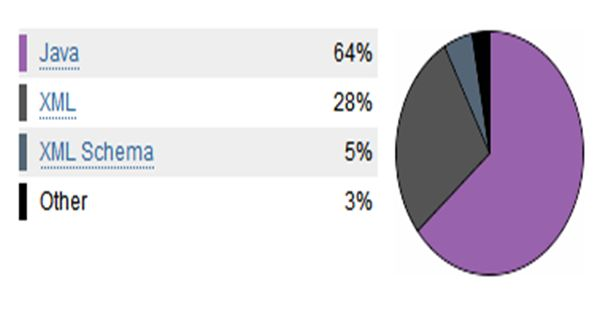
\includegraphics [scale=0.9] {codedistribution.jpg}
  \caption[Code Distribution Geotools]{Code distribution in Geotools}
\end{center}
\end{figure}

\begin{itemize}
\item Raster formats and data access
\item Arcsde, arcgrid, geotiff, grassraster, gtopo30, image (JPEG, TIFF, GIF, PNG), imageio-ext-gdal, imagemoasaic, imagepyramid, JP2K, matlab
\item Database “jdbc-ng” support
\item Db2, h2, mysql, oracle, postgis, spatialite, sqlserver
\item Vector formats and data access
\item App-schema, arcsde, csv, dxf, edigeo, excel, geojson, org, property, shapefile, wfs
\item XML Bindings
\item Java data structures and bindings provided for the following: xsd-core (xml simple types), fes, filter, gml2, gml3, kml, ows, sld, wcs, wfs, wms, wps, vpf.
\item Additional Geometry, Filter and Style parser/encoders available for DOM and SAX applications.
\end{itemize}

\section{Tools Used}

\subsection{Netbeans 7.0.1}
NetBeans IDE 7.0.1 includes the following notable changes:

\begin{itemize}
\item Full JDK 7 support: Running NetBeans IDE on top of JDK 7 and support for the final version of the JDK 7 language features
\item Integration of the recent patches
\item Performance improvements
\end{itemize}

\subsubsection{JDK 7}
\begin{itemize}
\item Project Coin support
\item Editor enhancements: Code completion, hints
\end{itemize}
\subsubsection{WebLogic Server}
\begin{itemize}
\item Streamlined and faster deployment to WebLogic
\item New server runtime node displaying deployed applications and resources
\item JSF integration with server libraries
\end{itemize}
\subsubsection{Oracle Database}
\begin{itemize}
\item Simplified connection wizard
\item Guided installation to JDBC driver
\item Editing and deployment of stored procedures
\end{itemize}
\subsubsection{GlassFish}
\begin{itemize}
\item GlassFish 3.1 support
\item Domain restart and log viewer for remote GlassFish
\item Enable and disable deployed applications
\end{itemize}
\subsubsection{Java}
\begin{itemize}
\item Maven 3 support
\item JUnit 4.8.2 integration and various JUnit improvements
\item Remote HTTP URLs supported for Javadoc in libraries and Java platforms
\item New improved visual customizer for GridBagLayout
\end{itemize}
\subsubsection{Java EE}
\begin{itemize}
\item Improved support for CDI, REST services and Java Persistence
\item New support for Bean Validation
\item Support for JSF component libraries, including bundled PrimeFaces library
\item Improved editing for Expression Language in JSF, including code completion, refactoring and hints
\end{itemize}
\subsubsection{Web Languages}
\begin{itemize}
\item HTML5 editing support
\item JSON formatter
\end{itemize}
\subsubsection{PHP}
\begin{itemize}
\item Generate PhpDoc
\item Rename refactoring, Safe Delete Refactoring
\item PHP 5.3 - Support for aliases
\end{itemize}
\subsubsection{C/C++}
\begin{itemize}
\item Easy import of project from user's existing binary
\item New Project type where user's source files are located on remote system
\end{itemize}
\subsubsection{NetBeans Platform}
\begin{itemize}
\item Annotations for generating Action registrations in the layer
\item Performance enhancements \& tight integration with Profiler
\item Additional NetBeans API changes
\end{itemize}
\subsubsection{General}
\begin{itemize}
\item Word wrap in Editor
\item Enhanced Profiler integration
\item Less intrusive checking for external changes when switching between the IDE and other programs.
\end{itemize}

\chapter{Summary and Conclusion}

\section{Summary}
Summary of activities carried out during major project training at BISAG can be listed as below:
\begin{itemize}
\item Initial Learning about the technologies and  the tools.
\item Requirement Analysis of the project.
\item Project Design including GUI related  design.
\item Project Development (Coding).
\item Testing  of the project.
\item Quality Related Work
\item Final  Documentation.
\end{itemize}

\section{Conclusion}
In "Desktop GIS Application" various functionalities of GIS are implemented. Various classes are given in Geotools which is used to make this software. Many classes are already available in Geotools using which functionalities such as navigation, quering, finding, selection, saving and croping like functionalities
are developed in this project.
